\chapter {Náhodné siete}

Keď jednotlivým uzlom v sieti necháme voľnosť pri výbere kvórových rezov výsledná
sieť môže vyzerať rôzne. Keď necháme sieť organicky sa vyvíjať v reálnom svete
ukazuje sa, že sieť skončí viac či menej centralizovaná alebo naopak náhodná,
v ktorej ťažko hľadať pravidlá a zákonitosti podľa ktorých sa bude sieť vyvíjať
ďalej, poprípade ktoré uzly majú väčšiu váhu pri rozhodovaní siete o novom bloku.

\textit{Reťazové} siete z minulej kapitoly boli príkladom siete, ktorá skončila
centralizovaná, presnejšie závislá len na niekoľkých uzloch.
Pokiaľ sieť naozaj vznikala organicky bez vonkajších zásahov
(každý uzol si zvolil kvórové rezy podľa seba), tak tieto uzly na ktorých závisí 
sieť majú na jednej strane zdravo vybudovanú autoritu a teda predpoklady byť
naozaj dôveryhodné, no pokiaľ ich je málo znižujú bezpečnostný koeficient.

V tejto kapitole sa preto budeme venovať druhému zaujímavejšiemu prípadu.
A to sieťam, kde kvórové rezy budú generované náhodne. Pokúsime sa najskôr
nagenerovať niekoľko takýchto sietí a následne zrátať ich koeficienty odolnosti.
Aby sme vedeli ale robiť niektoré porovnania medzi jednotlivými sieťami a zamedziť
veľa prípadom kde sieť má bezpečnostný koeficient 0 (tieto prípady sú nezaujímavé,
keďže v praxi sú tieto siete nepoužiteľné) budeme uvažovať len
\textit{zjednodušené NQK-siete}.

\section {Generovanie sietí}

Na generovanie sietí, konkrétne kvórovej funkcie, sme vytvorili program, ktorý ako
parameter berie typ siete ktorý má vytvoriť. Podporuje typy: \uv{chain}
(reťazová sieť), \uv{cyclic} (cyklická sieť) a \uv{random} (náhodná sieť).
Aby bolo jednoduché doplniť prípadné generovanie aj iných typov sietí, na samotné
naprogramovanie sme použili návrhový vzor \uv{Stratégia}\cite{gamma1995design}.

Následne po spustení programu je možné na vstupe zadať $N, Q, K$ -- parametre
zjednodušenej NQK-siete.
Pri generovaní náhodnej siete sme na generovanie náhodných kvórových rezov použili
Fisher-Yatesov algoritmus\cite{fisher1943statistical}, ktorým sme pre každý uzol
vytvorili náhodnú permutáciu ostatných uzlov a všetky $K$-prvkové podmnožiny
prvých $Q$ uzlov sme oznčili za jeho vlastné kvórové rezy.\\
Samotný program na generovanie sietí je priložený v prílohe.

\section {Hľadanie bezpečnostného koeficientu}

Na nájdenie tohto koeficientu potrebujeme nájsť veľkosť najmenšieho prieniku kvór.
Ako sme ukázali tento problém je NP-ťažký, preto podobne ako pri generovaní sietí
sme naprogramovali pomocou \textit{Stratégie} viac možných postupov ako tento
prienik nájsť.
Algoritmus na hľadanie sa skladá z dvoch častí, z hľadania kvór a následne
najmenšieho prieniku medzi ľubovoľnými dvoma z nich.

Na hľadanie kvór sme naprogramovali tri stratégie:

\begin{itemize}
  \item \textit{all} -- pozrie sa na každú podmnožinu a overí, či je to kvórum
  \item \textit{minimal} -- rovnako ako stratégia \textit{all}, ale ak už je niektorá
                            podmnožina kvórum, tak jej nadmnožiny už neoveruje,
                            teda nájde len minimálne kvóra
  \item \textit{random} -- predchádzajúce stretégie generujú všetky podmnožiny a preto
                           sú nepoužiteľné na väčších sieťach, preto táto stratégia
                           skúsi nájsť aspoň niekoľko náhodných kvór
\end{itemize}

Použitie stratégie si môžeme zvoliť parametrom pri spúštaní programu.
Overiť či je podmnožina kvórum je jednoduché, stačí overiť, či existuje kvórový rez
každého vrchola taký, že aj on je celý v danej podmnožine.

Stratégia \textit{random} postupuje tak, že sa spustí niekoľko krát.
Na začiatku každého spustenia si náhodne určí štartovací vrchol a udržuje si aktuálnu
množinu uzlov $Q$, v ktorej máme na začiatku iba štartovací vrchol.
Následne sa snaží množinu $Q$ \uv{rozširovať} pokým netvorí kvórum.

Rozširovať sa ju snaží nasledovne. Udržuje si množinu $A$ ešte nespracovaných uzlov
(takých čo ešte nemajú celý kvórový rez v $Q$) v ktorej je na začiatku len štartovací
vrchol.
Pokým je $A$ neprázdna vyberieme z nej ľubovoľný prvok $a$ a snažíme sa do $Q$ pridať
niektoré uzly, tak aby niektorý kvórový rez $a$ bol obsiahnutý v $Q$. Keďže naša sieť
je \textit{NQK-sieť}, tak len vyberieme našich $Q_a$ dôveryhodných uzlov a stačí nám
do $Q$ pridať $K_a$ uzlov odtiaľto. Algoritmus vždy vyberie všetky uzly, ktoré už
v $Q$ sú (nebudeme zbytočne zväčšovať kvórum). A pokiaľ ich ešte nie je dosť, náhodne
vyberie ďalšie a tie pridá do $A$ aj do $Q$. Teraz už uzol $a$ má kvórový rez v $Q$
a môžeme ho vymazať z $A$. Takto keď vyprázdnime $A$, tak z $Q$ už budeme mať určite
kvórum a náš program môžeme zopakovať a hľadať iné kvórum. Zjavne každý uzol bude v $A$
najviac raz, takže algoritmus sa nezacyklí.\\
Pre detajly uvádzame aj pseudokód \ref{alg:randomstrategy} na nájdenie jedného kvóra,
keď ich chceme nájsť viac spustíme tento algoritmus viac krát.

\begin{algorithm}
\caption{Hľadanie jedného kvóra stratégiou random}\label{alg:randomstrategy}
\begin{algorithmic}[1]
\State $\textit{v} \gets \text{náhodný začiatočný uzol}$
\State $Q \gets \{v\}$
\State $A \gets \{v\}$
\While{A je neprázdne}
  \State $a \gets$ ľubovoľný uzol z $A$
  \State $kandidati \gets$ všetky dôveryhodné uzly uzla $a$ nenachádzajúce sa v $Q$
  \If {$K_a > Q_a - |kandidati|$}
    \State $noveUzly \gets$ náhodných $K_a - Q_a + |kandidati|$ uzlov z množiny $kandidati$
    \State $Q \gets Q \cup noveUzly$
    \State $A \gets A \cup noveUzly$
  \EndIf

  \State $A \gets$ $A \setminus\{a\}$
\EndWhile
\State \textbf{return} $Q$
\end{algorithmic}
\end{algorithm}

Keď už máme nájdený neaký zoznam kvór (či už všetky alebo aspoň niekoľko náhodných),
tak ešte musíme zistiť ich najmenší prienik. To budeme robiť jednoducho a teda tak,
že porovnáme každé kvórum s každým, zrátame počet spoločných uzlov a zistíme
najmenší výsledok.\\
Samotný kód v C++ sa nachádza v prílohe.

\section {Exaktné výsledky}

Najprv sa skúsime pozrieť na siete, ktorým vieme zrátat bezpečnostný koeficient
exaktne. 
Aj keď stratégia \textit{minimal} je rýchlejšia ako \textit{all}, keďže nekontroluje
úplne všetky podmnožiny, tak nie je použiteľná na siete s vysokým počtom uzlov.
Môže sa totiž stať že bude musieť kontrolovať takmer každú podmnožinu.

Vygenerovali sme si teda \textit{zjednodušené NQK-siete} s parametrami
$2\leq N\leq 17,$\\
$1\leq Q < N, 1\leq K\leq Q$, pričom z každej trojice parametrov
spĺňajúcich tieto obmedzenia sme vygenerovali 5 náhodných sietí (teda pre každý
uzol náhodné kvórové rezy).

\begin{figure}
\centerline{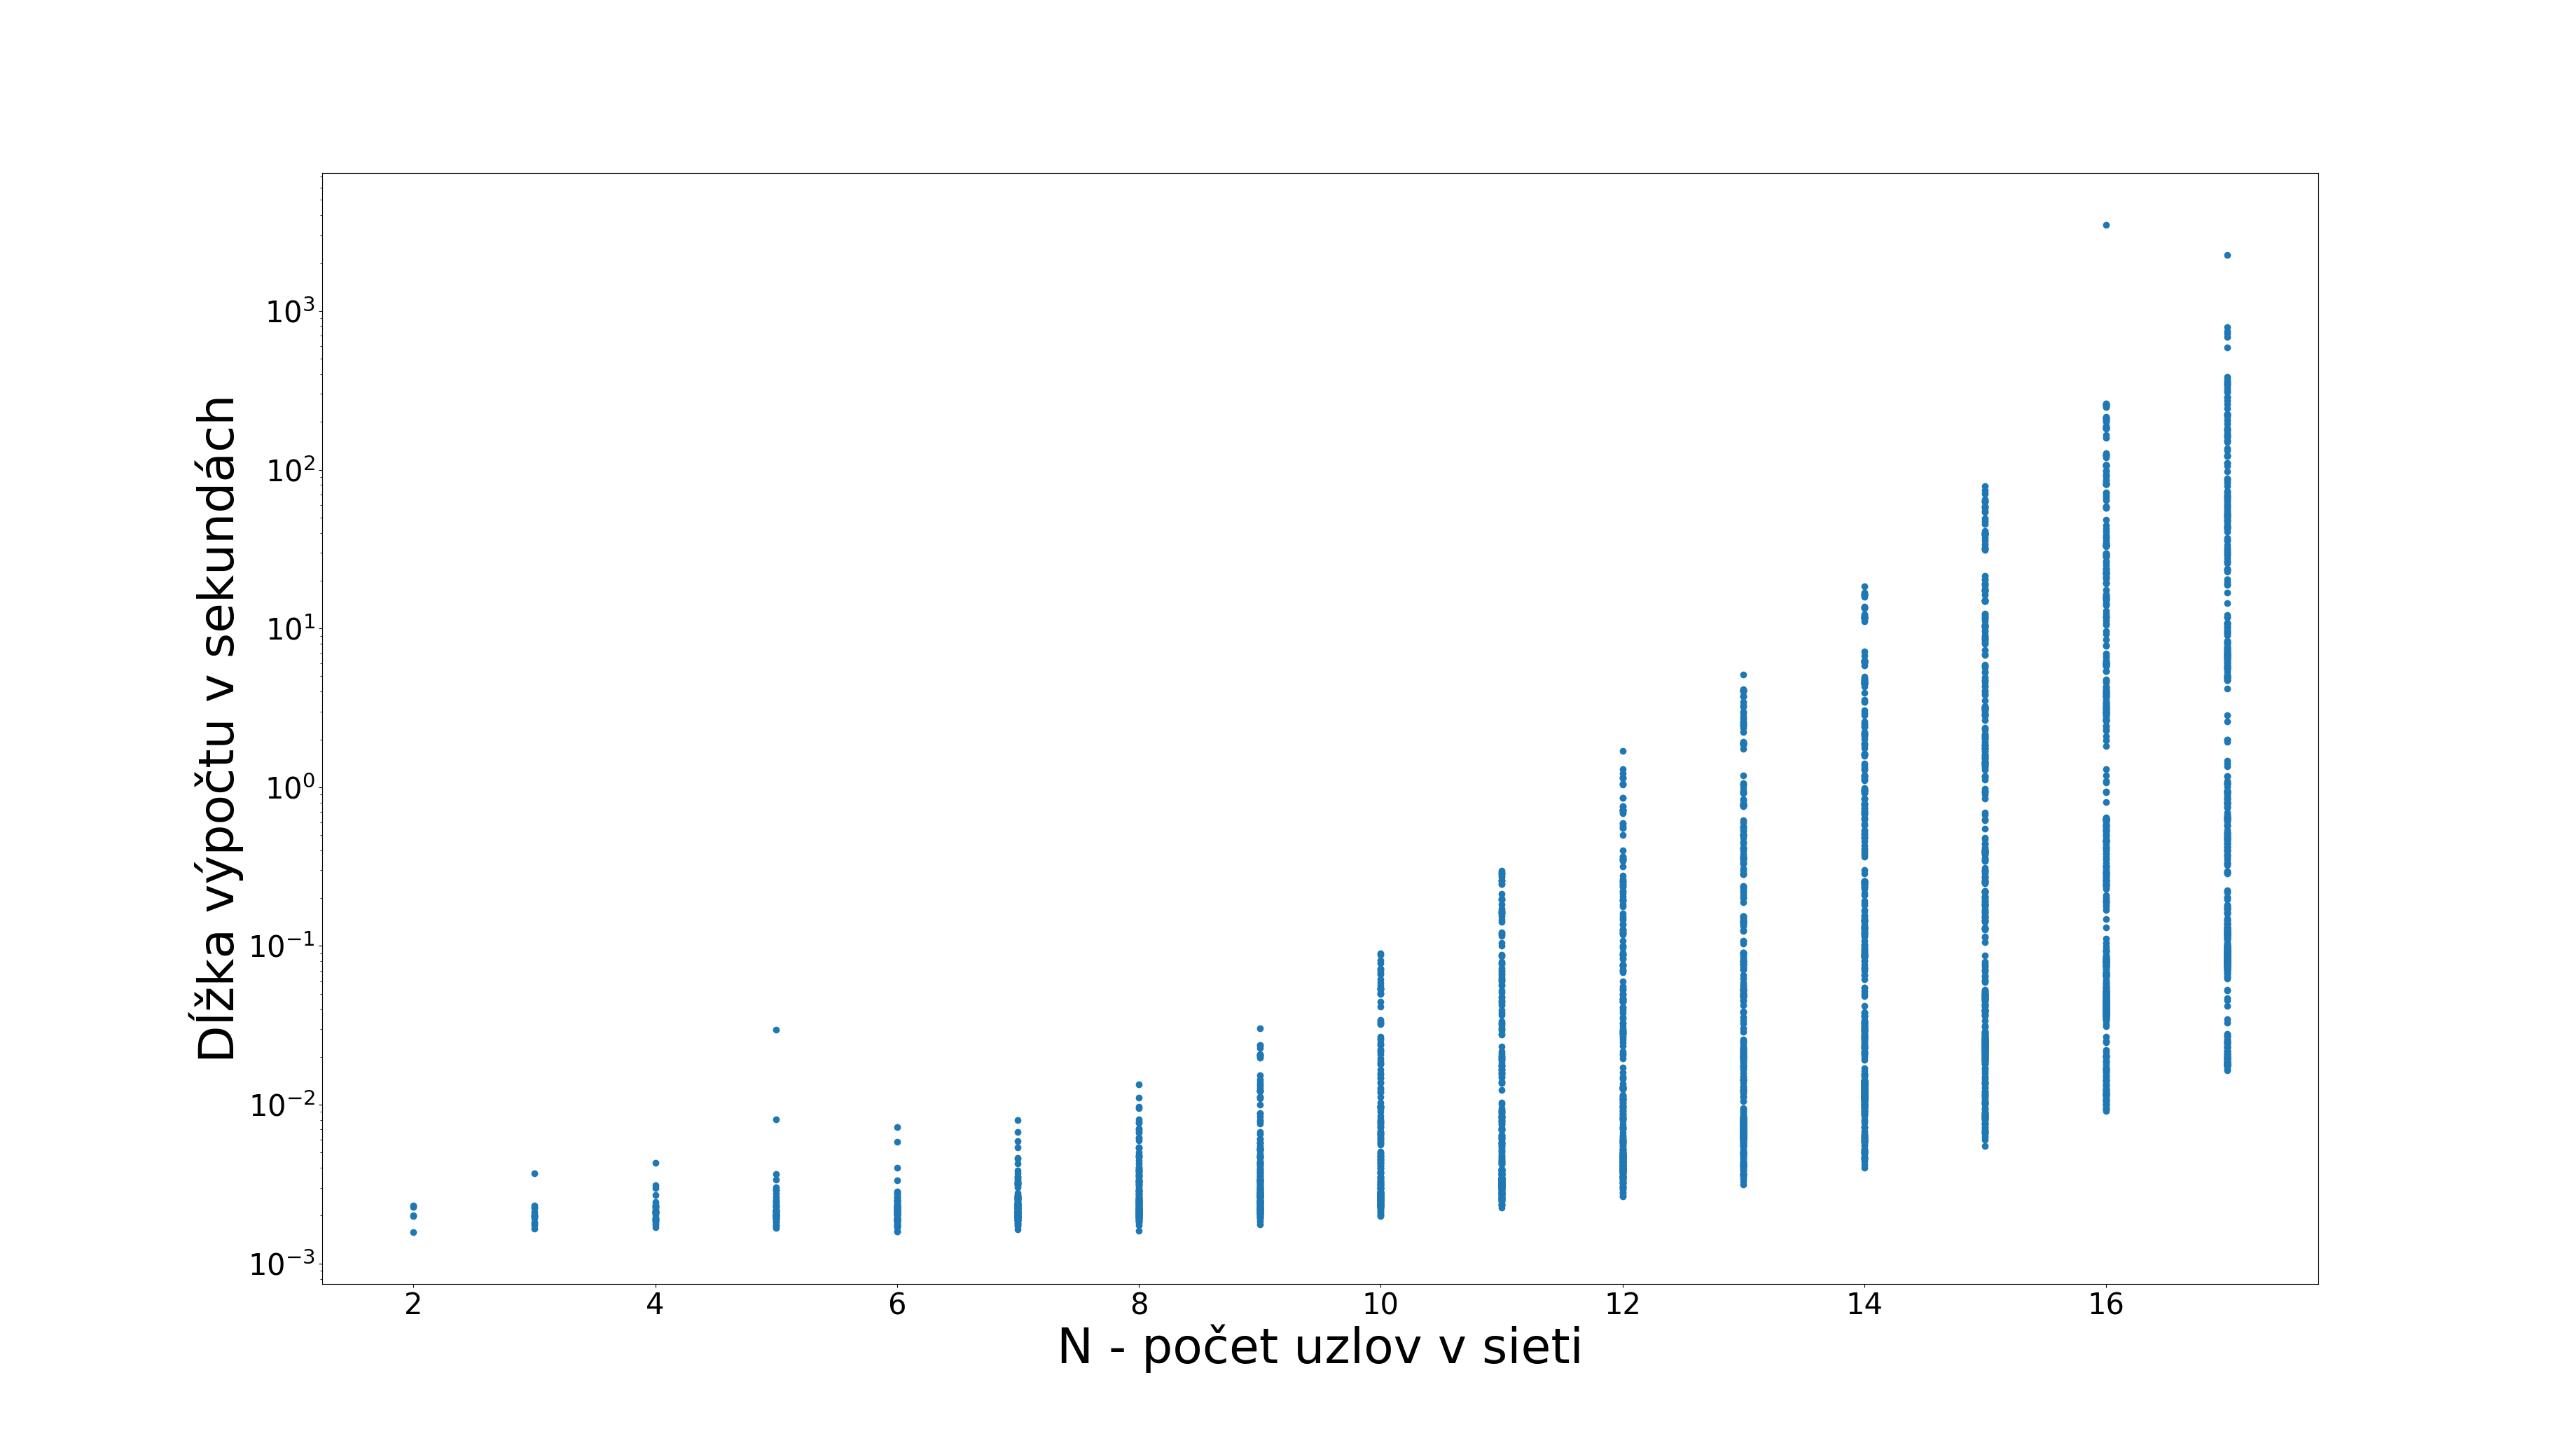
\includegraphics[width=1.2\textwidth]{images/cas_ku_N.png}}
\caption{Graf rastu dĺžky výpočtu algoritmu od veľkosti siete} \label{obr:cas_velkost}
\end{figure}

Ako si môžeme všimnúť na grafe \ref{obr:cas_velkost} čas výpočtu nášho algoritmu
v najhoršom prípade exponenciálne rastie s počtom uzlov v našej sieti. Pre 17 uzlov
v sieti algoritmus niekedy potrebuje $10^3$ sekúnd, čo je zhruba 15 minút. Preto sme
už pre väčšie siete nedokázali analyzovať exaktné výsledky. Všimnime si, že naopak
niektoré siete s 17 uzlami sme boli schopný analyzovať celkom rýchlo pod sekundu.
Je to spôsobené našou stratégiou, ktorá závisí od veľkosti minimálnych kvór. Totiž
ak má sieť malé kvóra nemusíme kontrolovať väčšie nadmnožiny a algoritmus je rýchlejší.
Avšak vidno, že aj rýchlosť algoritmu v najlepšom prípade tiež rapídne rastie
(y-ová os rastie logaritmicky).

\begin{figure}
\centerline{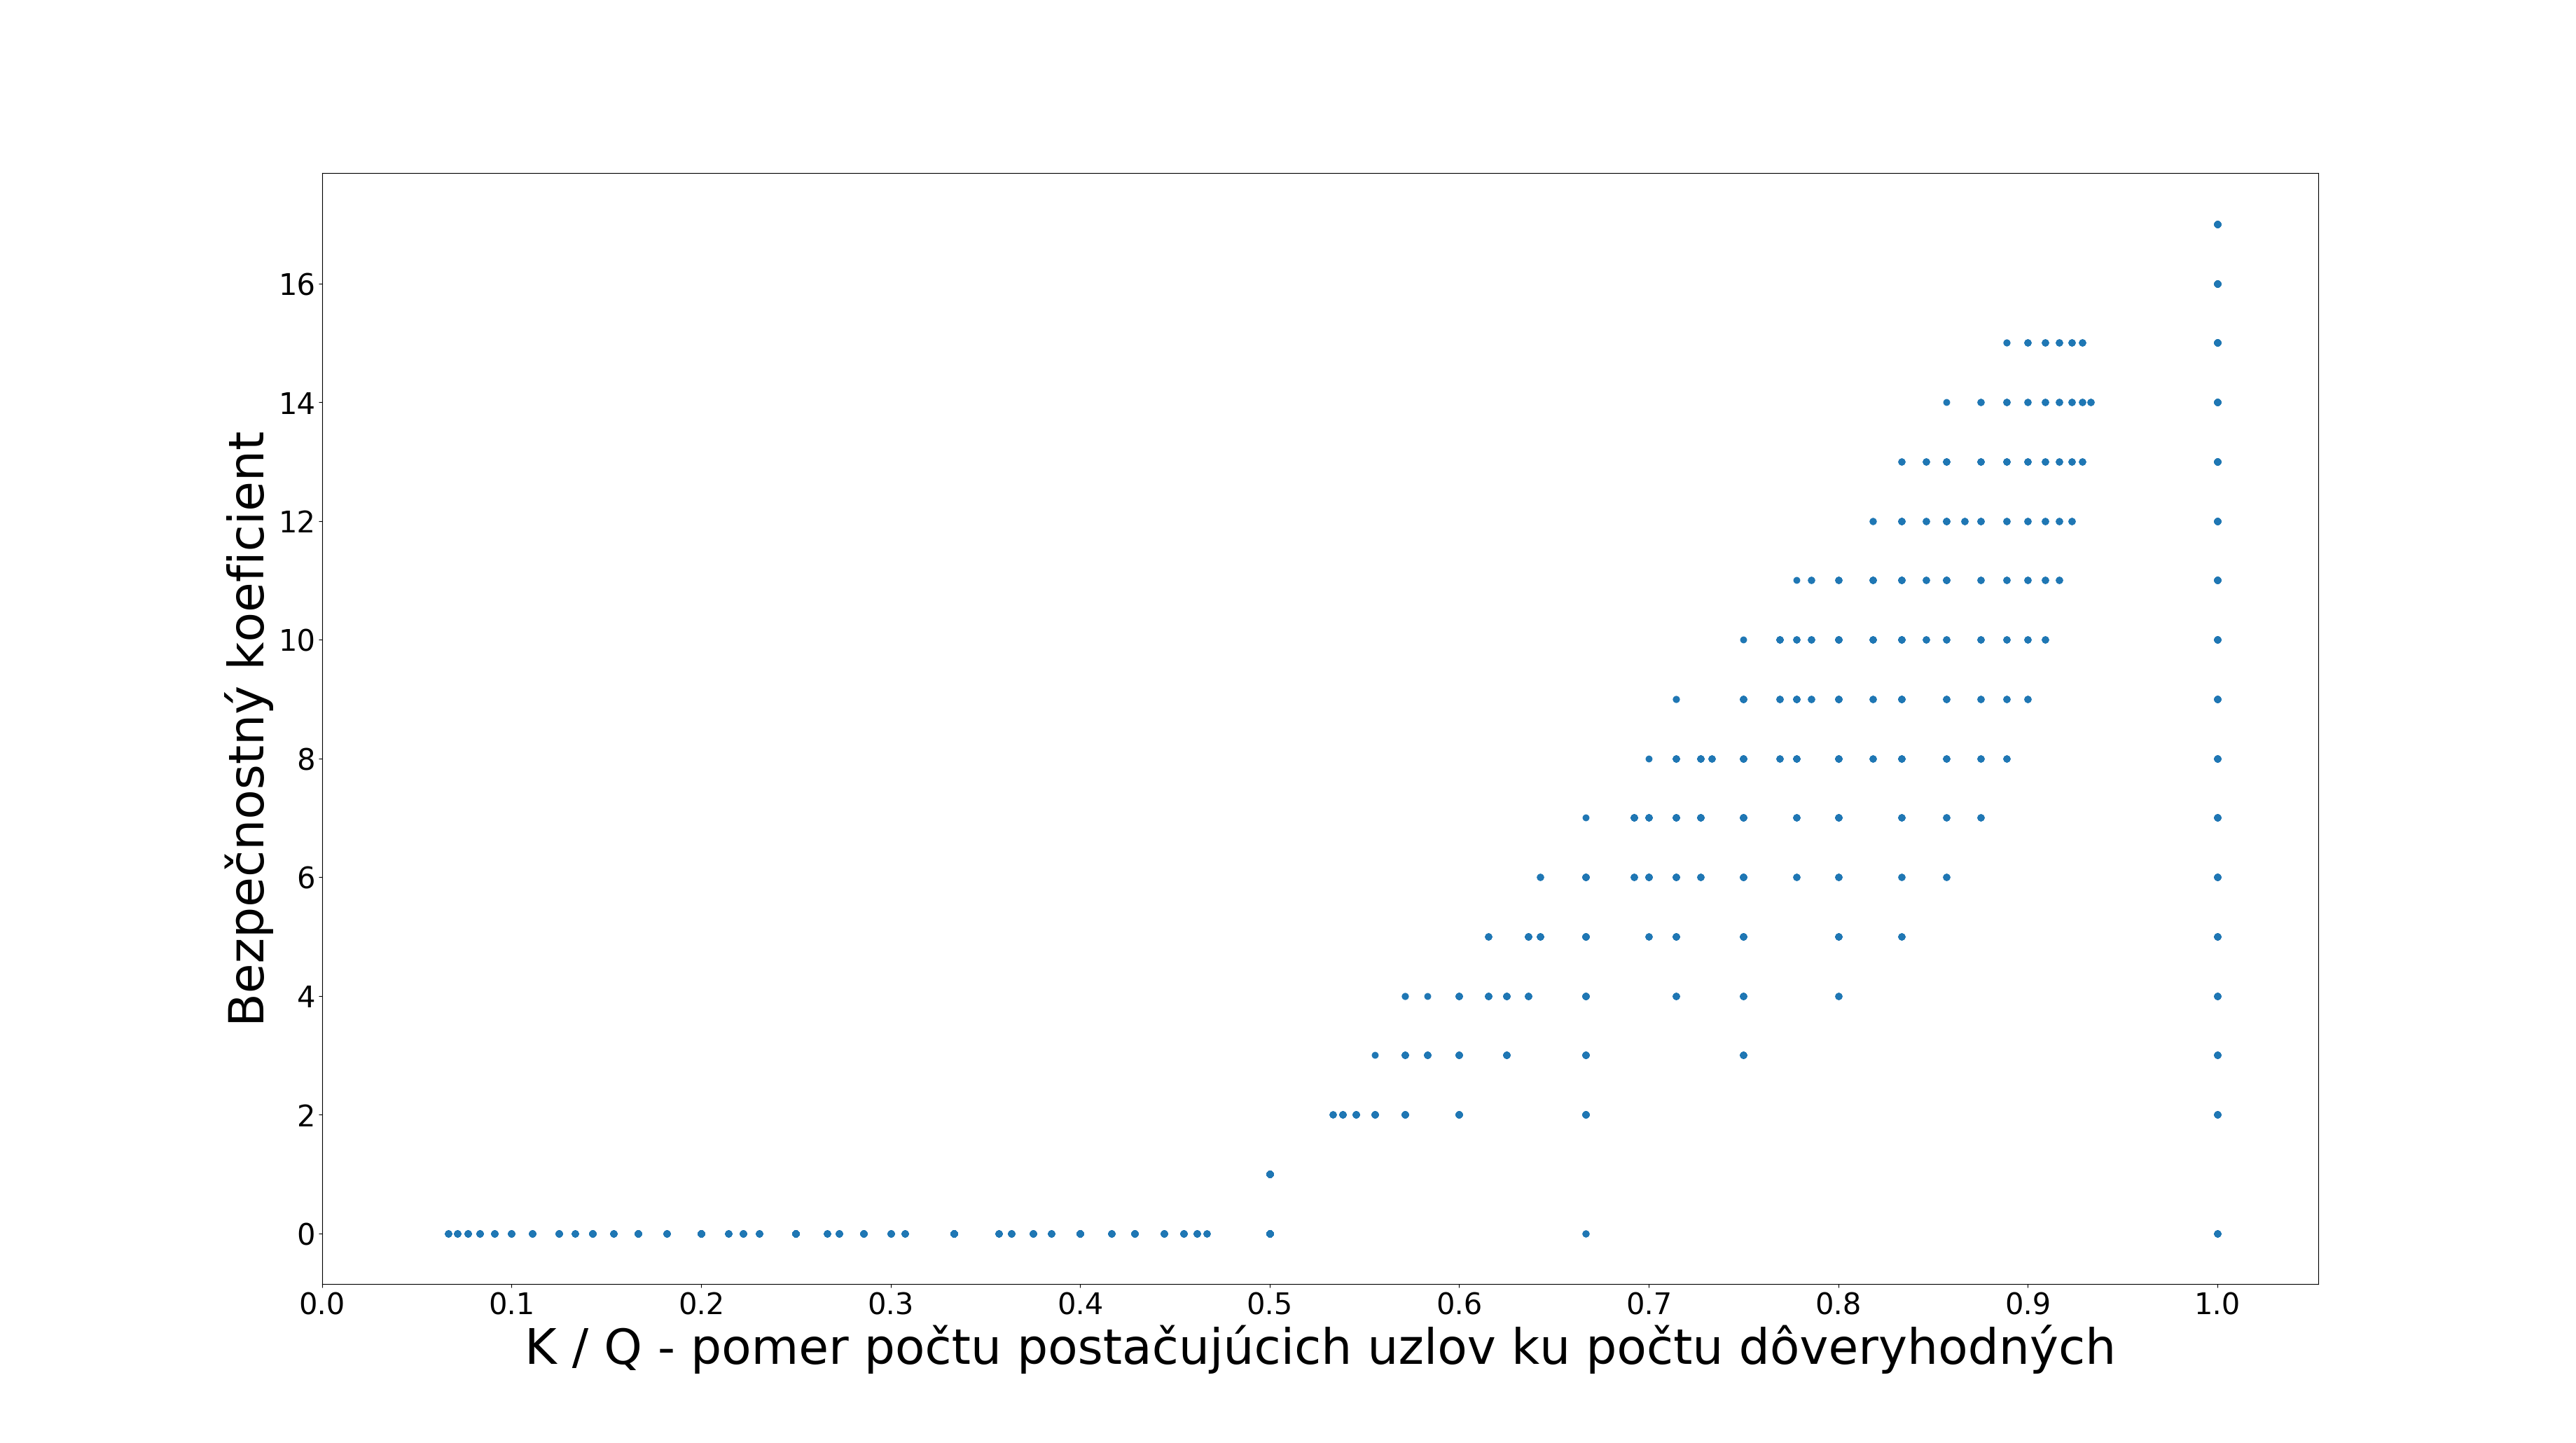
\includegraphics[width=1.2\textwidth]{images/KkuQ_prienik.png}}
\caption{Graf vzťahu pomeru K ku Q a bezpečnostného koeficientu} \label{obr:KkuQ_bezpecnost}
\end{figure}

Analýzu týchto malých sietí, ktoré sme boli schopný exaktne spočítať začneme
grafom \ref{obr:KkuQ_bezpecnost}, ktorý ukazuje aký bezpečnostný
koeficient majú jednotlivé siete vzhľadom na pomer parametrov $K$ a $Q$.
Môžme si všimnúť, že graf má akokeby 3 časti.
Prvá časť sú siete v ktorých je $K$ príliš malé vzhľadom na $Q$. Presnejšie
ak $K < Q/2$, tak medzi nami vygenerovanými sieťami žiadna nemala prienik kvór.
Z čoho dostávame, že nie sú bezpečné a teda sú v praxi nepoužiteľné a pre nás
nezaujímavé. Naše dáta sú síce veľmi malé siete, no môžeme vysloviť hypotézu,
že siete s $K < Q/2$ nebudú nikdy bezpečné a teda môžeme neodporučiť uzlom voliť
takéto kvórové rezy.
Na našu hypotézu sa ešte raz pozrieme v nasledujúcej podkapitole kde sa budeme
pozerať aj na väčšie siete hoci nebudeme vedieť určiť bezpečnostný koeficient
úplne presne, budeme vedieť spraviť aspoň horný odhad, ktorý pokiaľ bude nulový
bude aj presný.

Posledná časť grafu sú siete kde $Q=K$. Pokiaľ sa pozrieme na kvóra takýchto
vygenerovaných sietí, zistíme, že majú jediné kvórum a to všetky uzly, čo im
teda dá bezpečnostný koeficient rovný $N$, avšak koeficient životaschopnosti
bude $1$, čo výrazne obmedzuje odolnosť siete.
Určite jednoducho vieme zostrojiť aj siete tohto typu s viacerými kvórami.
Napriek tomu sme vygenerovali množstvo sietí (uvažujúc každý uzol za jedinečný,
každú sieť s rovnakou pravdepodobnosťou pri zadaných parametroch) a všetky boli
tohto typu, z čoho môžme usudzovať, že drvivá väčšina takto postavených sietí
skončí s jediným minimálnym kvórom.

Ostali nám len siete s $Q > K\geq Q/2$, ktoré na grafe vyzerajú už zaujímavejšie.
Môžme si všimnúť, že s rastúcim pomerom stúpa aj maximálny aj minimálny
bezpečnostný koeficient nájdený pre daný pomer (nemusí nutne stále rásť, ale
\uv{zhruba} rastie).
Pre takto vysoké pomery dokonca platí zaujímavá vlasnosť.

\paragraph{Veta}
V \textit{NQK-sieťach} s množinou uzlov $V$, ktoré majú prienik kvór je bezpečnostný
koeficient aspoň $\min\limits_{v\in V}2K_v-Q_v+1$.

\paragraph{Dôkaz}
Pre spor predpokladajme, že existuje menší prienik dvoch kvór.
Keďže takáto sieť má prienik kvór, tak existuje uzol $u$, ktorý sa nachádza v tomto
prieniku. Keďže $u$ patrí obom kvóram, tak obom kvóram patria aj po jednom z jeho
vlastných kvórových rezov. A to sú $K$--prvkové podmnožiny $Q$--prvkovej množiny uzlov
vybranej uzlom $u$. Všimnime si ale, že každé dve takéto podmnožiny majú prienik aspoň
$2K_u-Q_u$ uzlov, ktoré teda patria tiež obom kvóram. Teda náš uvažovaný prienik má
aspoň $2K_u-Q_u+1\geq\min\limits_{v\in V}2K_v-Q_v+1$ uzlov, čo je spor.$\blacksquare$

\vspace{3mm}
Pri štúdiu našich \textit{zjednodušených NQK-sietí}, teda máme že tento bezpečnostný
koeficient je aspoň $2K-Q+1$ (ak je nenulový). Týmto môžeme získať intuíciu rastu
minima bezpečnostného koeficientu medzi vygenerovanými sieťami s daným pomerom $K/Q$.
Keďže jednak pre zväčšujúci sa pomer, sa bude funkcia $2K-Q+1$ tiež zväčšovať a tiež
fixný menovateľ zlomku má len obmedzenú možnosť priblížiť sa 1 (najbližsie sa dostane pri
$\frac{Q-1}{Q}$), teda aj samotné $Q$ bude čoraz väčšie. Mohlo by sa teda zdať, že
najlepšie pre uzly je voliť $K$ blízke $Q$. Avšak v takýchto prípadoch klesá
\textit{koeficient životaschopnosti}.

\begin{figure}
\centerline{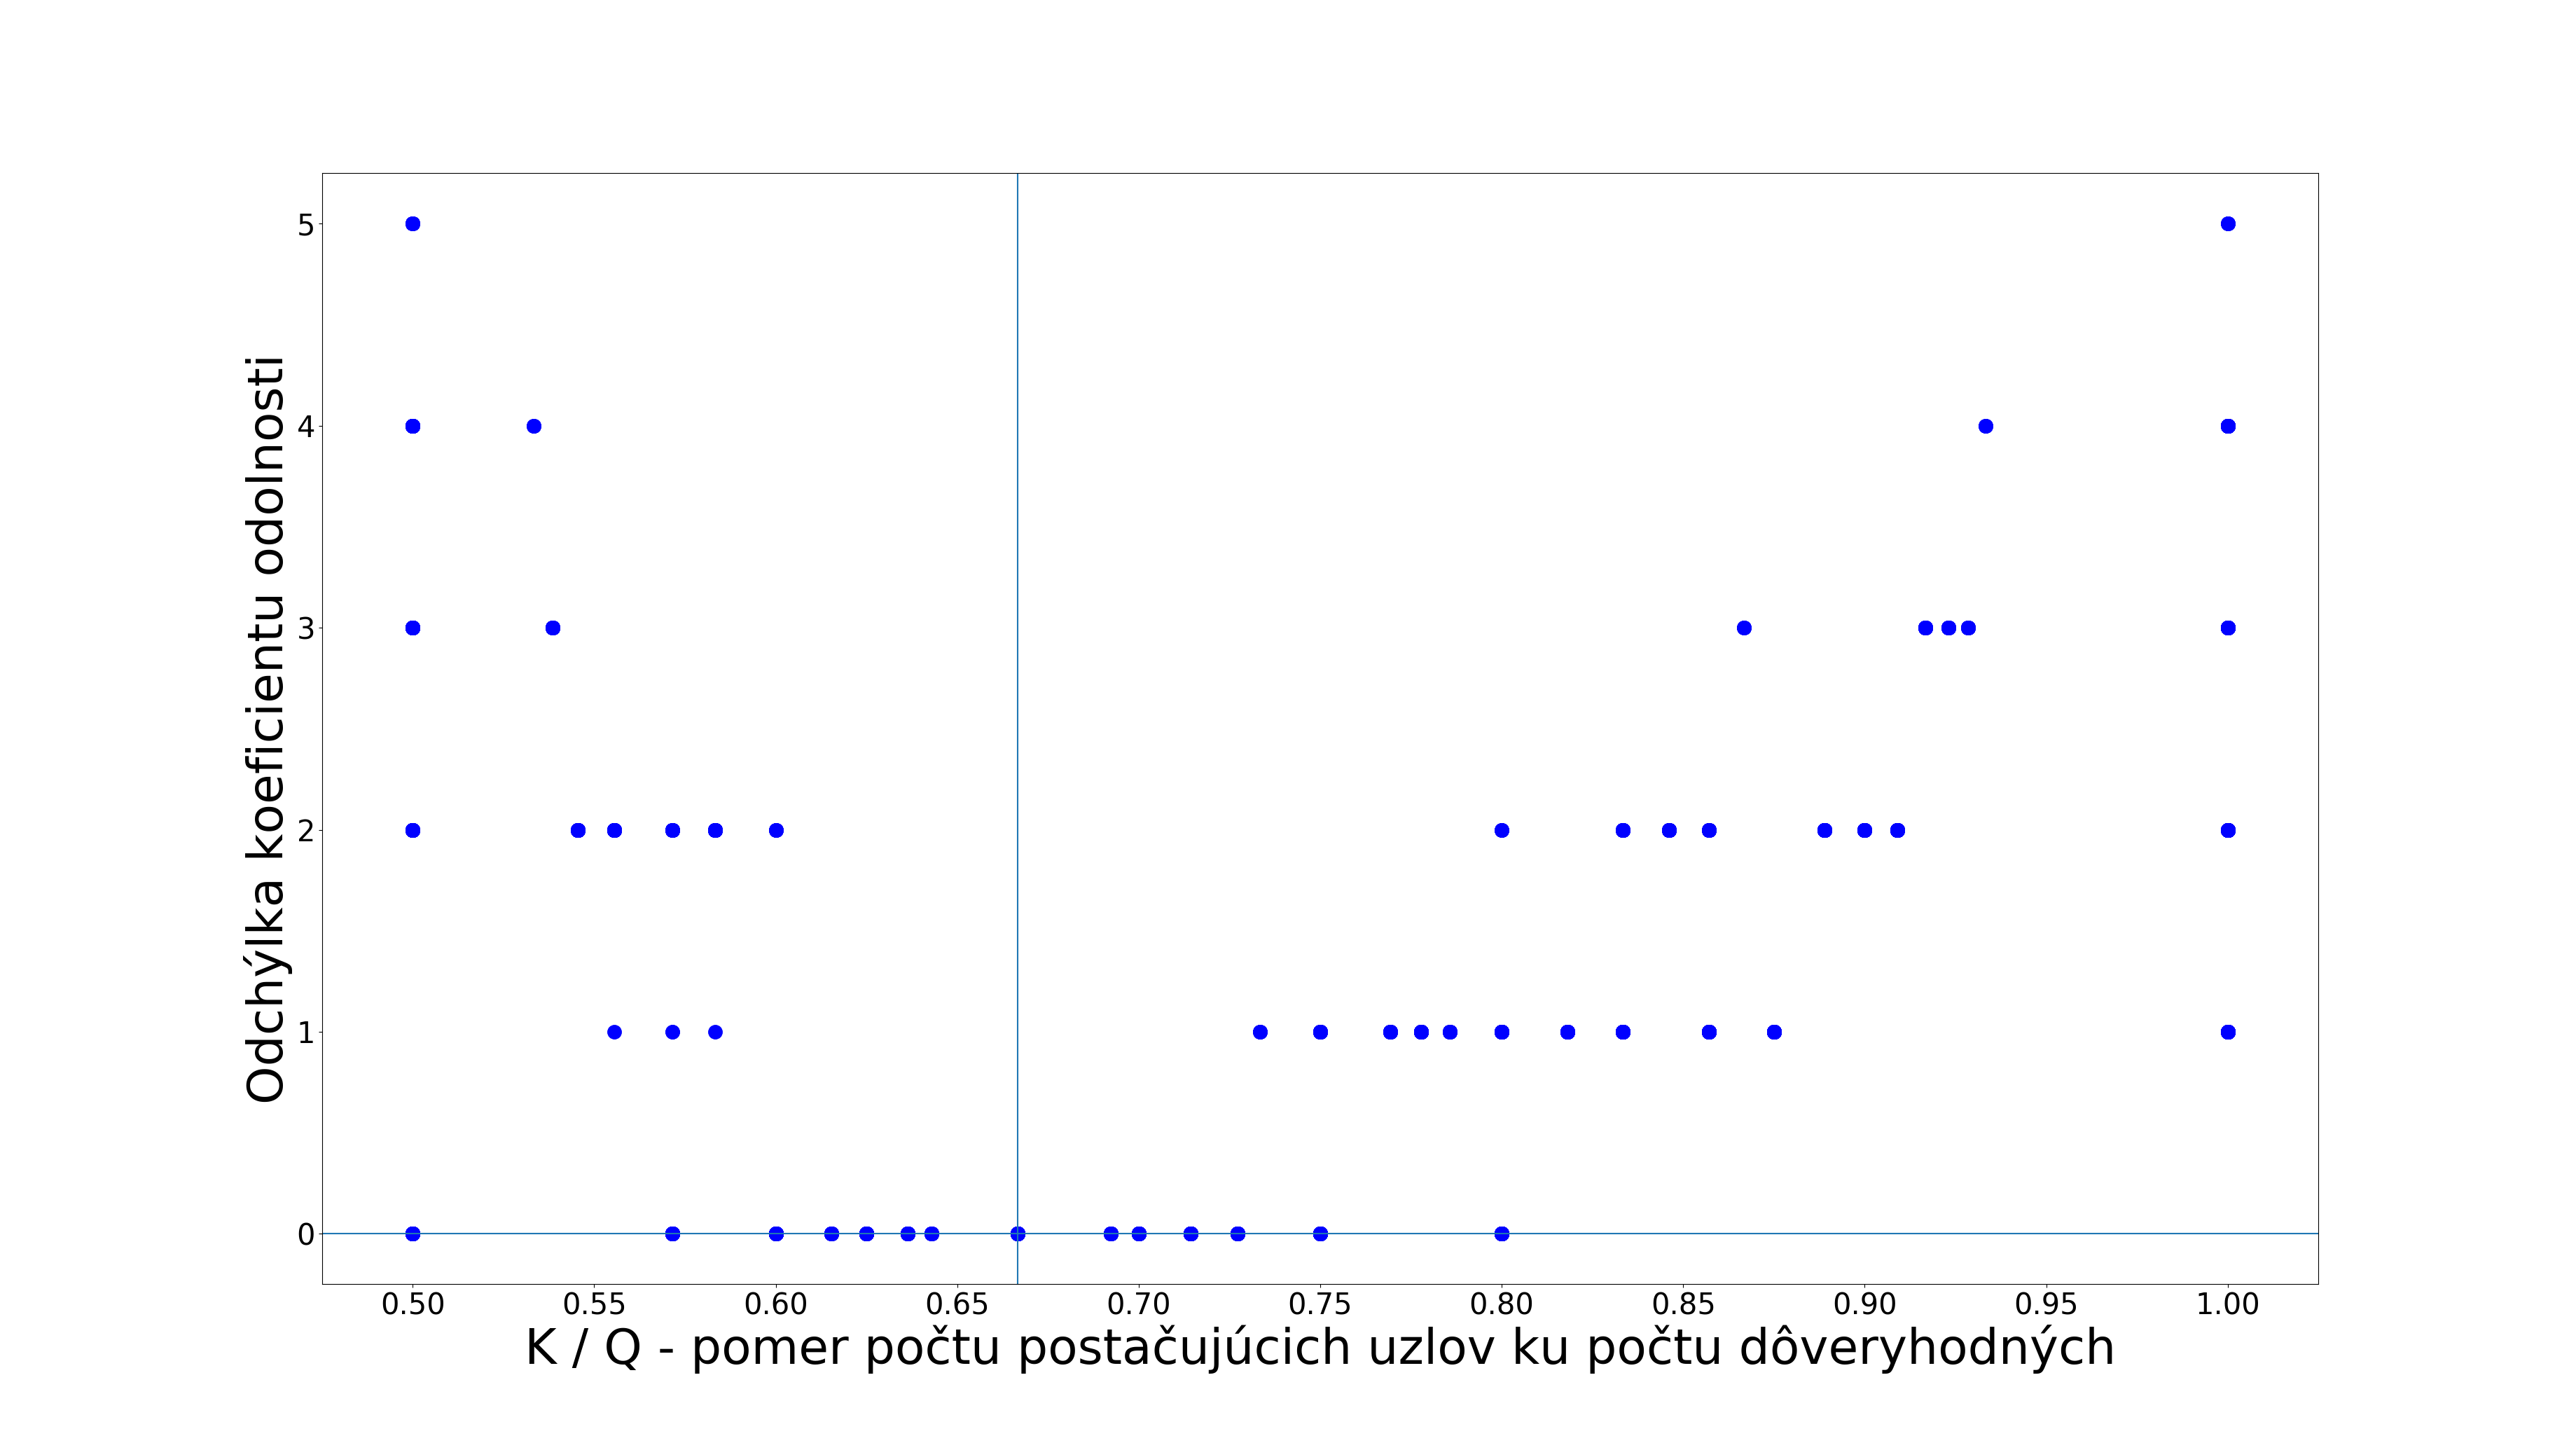
\includegraphics[width=1.2\textwidth]{images/KkuQ_odchylka.png}}
\caption{Graf odchýlky koeficientu odolnosti ku optimu} \label{obr:KkuQ_odchylka}
\end{figure}

Posledný odstavec boli len úvahy na vysvetlenie správania sa grafu
\ref{obr:KkuQ_bezpecnost}.
To čo je ale podstatné pre život siete je koeficient odolnosti. Ten vieme zrátať
jednoducho keď už máme bezpečnostný koeficient. Koeficient životaschopnosti
pre \textit{zjednodušené NQK-siete} sa ráta ľahko ako sme si už ukázali.
Keďže siete s $K < Q/2$ neboli bezpečné a použiteľné, tak ich v tejto úvahe
používať nebudeme.
Chceme zistiť ako voliť $K$ aby sieť dosiahla čo najväčší koeficient odolnosti.
Pomocou grafu \ref{obr:KkuQ_odchylka} si ukážeme, že ako najrozumnejšia
voľba sa ukazuje $K=\frac{2}{3}Q$.

Pre každú vygenerovanú sieť sme si vygenerovali jej \uv{optimálny} náprotivok,
teda sieť s rovnakými parametrami s tým, že $K=\frac{2}{3}Q$
($K=\lfloor\frac{2}{3}Q\rfloor+1$ ak by $K$ nevychádzalo celočíselné).
Vypočítali sme koeficienty odolnosti oboch sietí a do grafu zaznačili rozdiel
koeficientu pôvodnej siete od \uv{optimálnej}.

Ako si môžeme na grafe všimnúť naozaj všetky tieto rozdiely vyšli nezáporné
a teda sa nám podarilo potvrdiť na našich dátach optimálnosť voľby $K$.
Ďalšia zaujímavá vec je, že, keď vypočítame koeficient odolnosti na sieťach
s $K=\frac{2}{3}Q$, dostávame výsledky okolo $\frac{Q}{3}$, čo je veľmi
podobné s výsledkami v \textit{reťazových} sieťach.
Dokonca pokiaľ si zadefinujeme obdobné pojmy ako naše koeficienty v
centralizovanom Byzantínskom protokole\cite{li2007beyond}, získame presne
rovnaký pomer, ktorý musíme zvoliť aby sme získali rovnovážny stav medzi
obdobnými pojmami koeficientu životaschopnosti a bezpečnostného koeficientu
v tomto protokole. A ako výsledok dostaneme približne rovnakú odolnosť siete
(počet uzlov, ktorých môžu zlyhať a neovplyvní to chod siete).

\section {Horné odhady na koeficient odolnosti väčších sietí}

Teraz sa skúsime pozrieť aj na siete s väčším počtom uzlov, avšak už
na hľadanie bezpečnostného koeficientu budeme schopný požiť len stratégiu
\textit{random}. Tá však nemusí nájsť všetky kvóra a teda nebudeme schopný
určiť tento koeficient presne, ale budeme ho vedieť zhora ohraničiť,
keďže ak už neaký prienik kvór nájdeme, tak buď sme ešte neaký menší nenašli
alebo už menší neexistuje.

Vygenerovali sme si teda \textit{zjednodušené NQK-siete} s parametrami
$21\leq N\leq 50,$\\
$1\leq Q < N, 1\leq K\leq Q$, pričom parametre sme generovali tiež náhodne
a dokopy sme vygenerovali 200 sietí.
Ako hornú hranicu sme zvolili 50 aby sme jednak mali náš odhad celkom presný
(generovali sme 2000 náhodných kvór pre jednu sieť) a zároveň
dĺžka výpočtu bola únosná (väčšina výpočtov dokázala bežať do 15 sekúnd).

\begin{figure}
\centerline{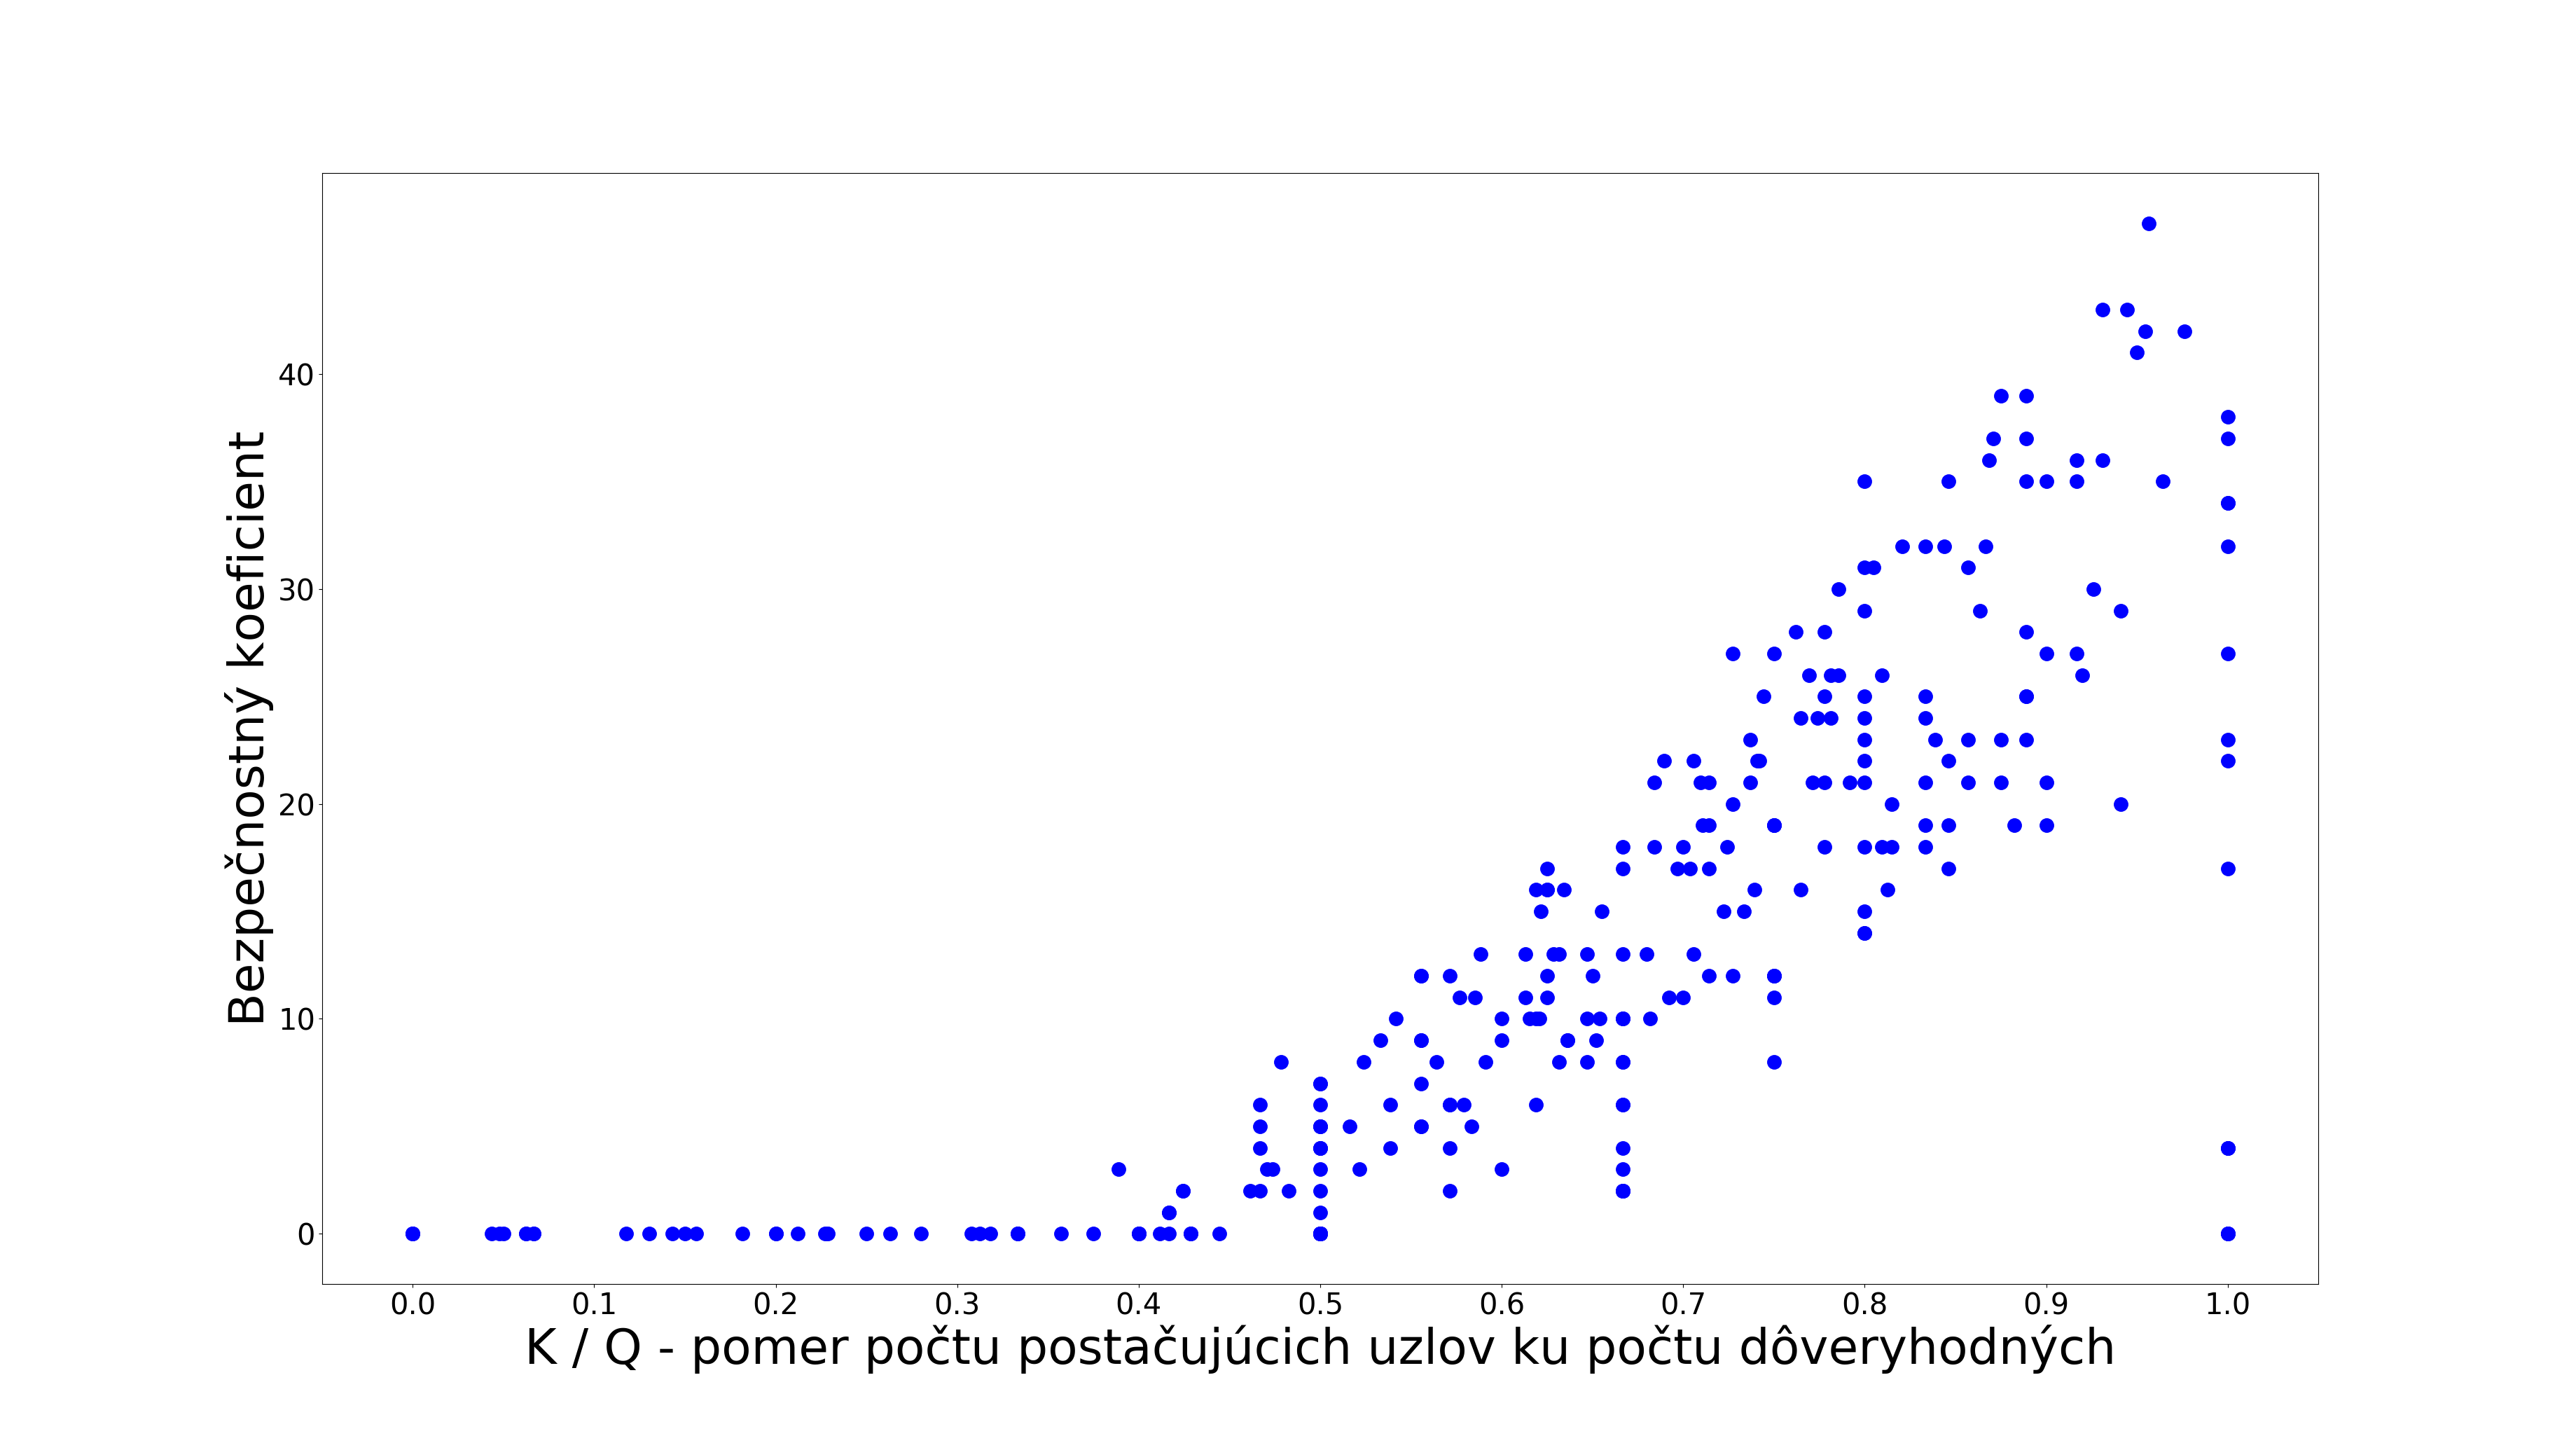
\includegraphics[width=1.2\textwidth]{images/KkuQ_prienik_large.png}}
\caption{Graf vzťahu pomeru K ku Q a bezpečnostného koeficientu veľkých sietí} \label{obr:KkuQ_bezpecnost_large}
\end{figure}

Najprv si skúsime vykresliť obdobný graf \ref{obr:KkuQ_bezpecnost_large} ako
pri malých sieťach a to vzťah medzi pomerom $K/Q$ a bezpečnostným koeficnetom.
Podobne ako v grafe \ref{obr:KkuQ_bezpecnost} tiež vidíme, že siete s
$K<\frac{Q}{2}$ majú poväčšine bezpečnostný koeficient nulový. Ešte by sme si
mali uvedomiť, že v grafe máme len horné odhady na bezpečnostné koeficienty,
teda reálne môžu byť aj nižšie. V každom prípade to potvrdzuje našu hypotézu
o tom, že voliť kvórové rezy tak, že $K<\frac{Q}{2}$ vedie k veľmi nízkemu
až nulovému koeficientu bezpečnosti a teda je dobré používať väčšie $K$.
Zvyšok grafu vyzerá veľmi podobne \ref{obr:KkuQ_bezpecnost}.
Môžme preto ľahko našu hypotézu rozšíriť aj na väčšie siete a predpokladať,
že bezpečnostný koeficient bude rásť podobne.
Čo nám dáva lepší odhad pri budovaní siete o jej bezpečnosti.

\begin{figure}
\centerline{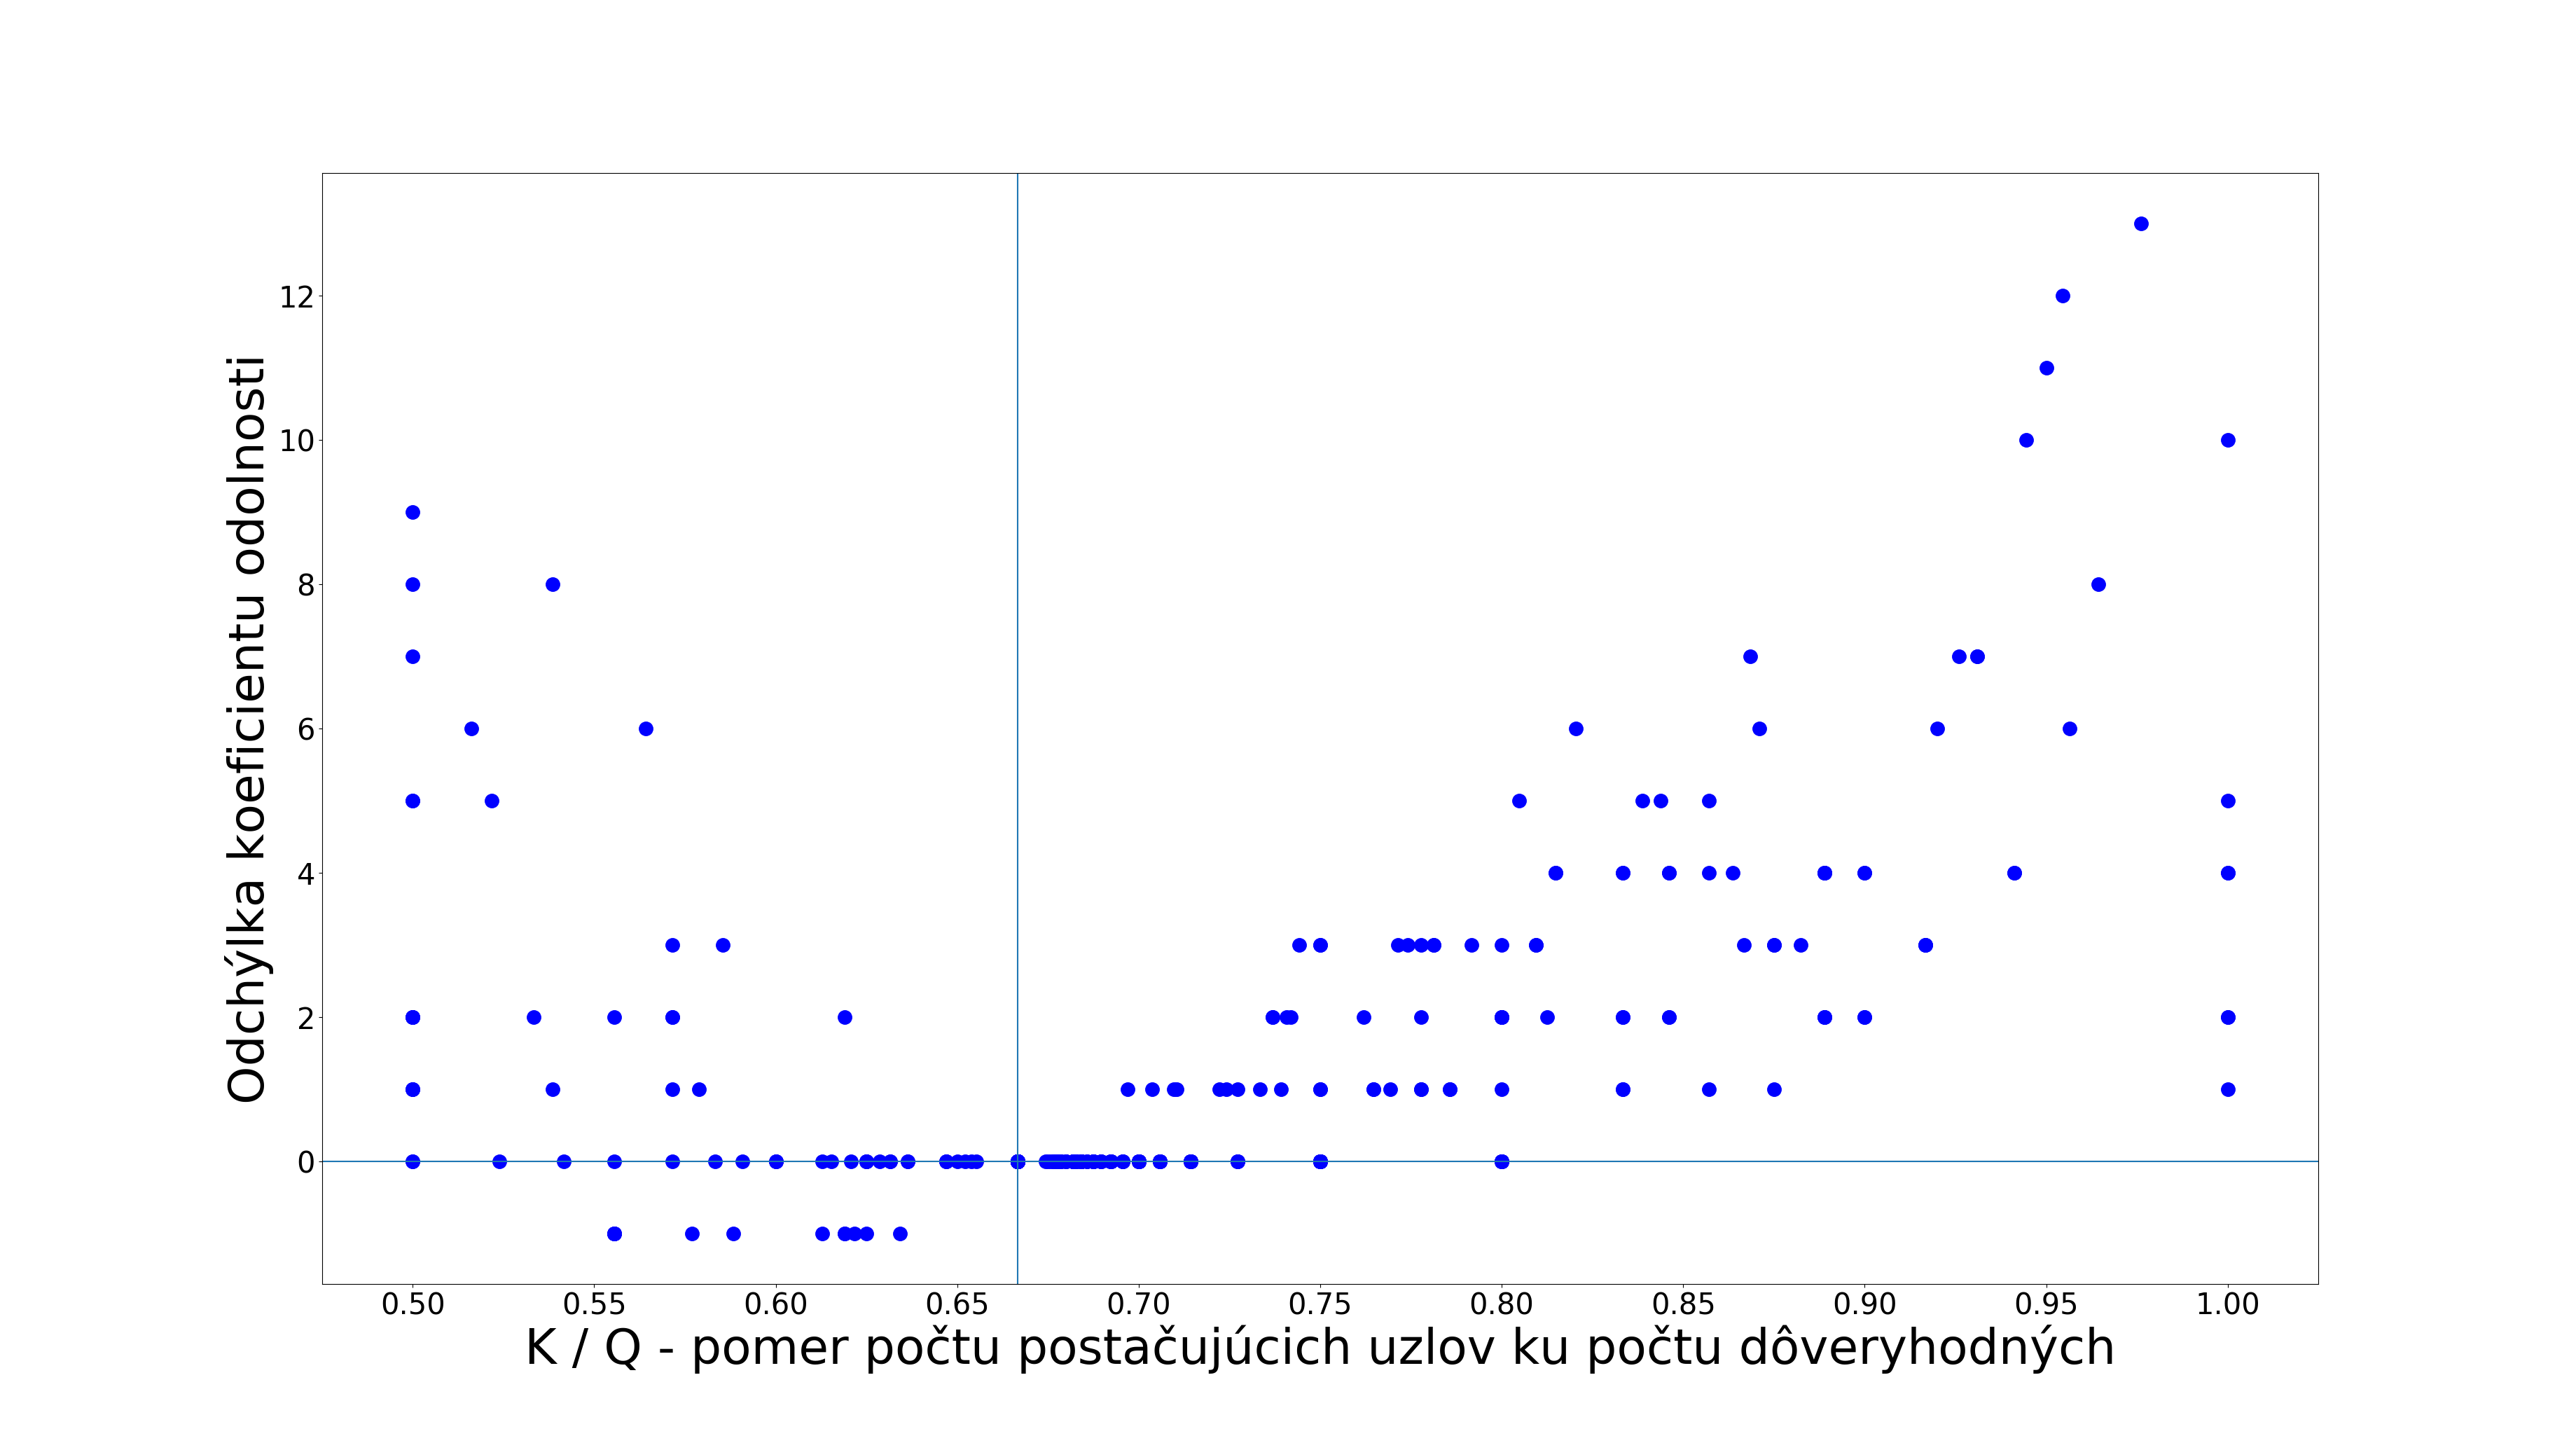
\includegraphics[width=1.2\textwidth]{images/KkuQ_odchylka_large.png}}
\caption{Graf odchýlky koeficientu odolnosti ku optimu vo väčších sieťach} \label{obr:KkuQ_odchylka_large}
\end{figure}

Na záver sa však pozrime na to najdôležitejšie a teda koeficient odolnosti.
Tu už takisto nebudeme uvažovať siete $K<\frac{Q}{2}$.
Podobne ako pri malých sieťach si vykreslíme rovnako stavaný graf
\ref{obr:KkuQ_odchylka_large}, na ktorého vybudovanie sme však použili vygenerované
väčšie siete a iba horný odhad bezpečnostného koeficientu a teda aj koeficientu
odolnosti.
Podobne ako pri malých sieťach sa nám znova potrvdzuje hypotéza o ideálnom
volení parametra $K$ v sieti, tak aby sme maximalizovali koeficient odolnosti.
Ukazuje sa nám, že pri mierne nižsom zvolení pomeru vieme získať o kúsok
väčší koeficient odolnosti (v našom prípade o 1), avšak bezpečnosť siete je oveľa
dôležitejšia ako samotná životaschopnosť a tak podobne ako v \cite{li2007beyond},
môžeme tvrdiť že predsalen je lepšie zvoliť pomer $\frac{2}{3}$. Pretože aj keď
celková odolnosť môže vyjsť o kúsok horšie, keďže bezpečnostný koeficient vyjde
lepšie \ref{obr:KkuQ_bezpecnost_large}, tak nepriateľ prinajhoršom iba zablokuje
sieť ale dáta v nej ostanú správne. A z tohto stavu je jednoduchšie sieť opraviť
a obnoviť jej prevádzku.\\
Čo však na tomto grafe vidno omnoho lepšie je, že čím viac sa vzďaľujeme od tohto
magického pomeru, tým viac sa naša odchýlka zväčšuje.
A teda najmä pri sieťach kde ťažko hovoriť o dôveryhodnosti konkrétnych uzlov
a akejkoľve dôležitosti uzla na protokol odporúčame uzlom voliť kvórové rezy
tak, aby počet postačujúcich uzlov ($K$) bol aspoň približne rovný $\frac{2}{3}$
počtu dôveryhodných uzlov ($Q$). Keďže ako sme ukázali to štatisticky vedie
ku sieti, ktorá je schopná prežiť najviac zlyhaných uzlov. Tak ako sme už uviedli
niekoľko krát vyššie, \textit{koeficient odolnosti} bude vychádzať okolo $\frac{Q}{3}$.